\newpage
\mysection{Commenting Code}

Comments are important! In academia, you think your professors are just trying to punish you, but we are giving you wisdom that we acquired. Un-commented programs are hard to read, even if written in your own hand. But let me give you a few more reasons to motivate you. 1) In industry, your comments will allow another programmer to read and understand your code much faster, besides the fact that poorly commented code will probably \textbf{get rejected} anyway by whatever system your company uses to manage versions or continuous integration. 2) Another factor is that since you have to post your code on Github, you want to put your best face forward when making your code publicly visible. Putting many well commented working programs on your Github repository will look good when you are applying for jobs. 3) Your grade in this course. I'll leave it at that, so, you might as well start commenting your code.\\


\mysubsection{Commenting Extremes}

The amount and style of comments is an entire subject that is debated to this day, and depending on the task (or workplace), you would vary the amount and style of your comments. Some extremes are: 1. no comments at all (competitive programming), 2. self documenting and 3. industry requirements. 

\mysubsubsection{Competitive Programming}

In competitive programming, you use short variable names, and short cryptic snippets of code that run fast with no need for an explanation. Why? It's all about a speedy solution at a competition. Comments are almost in the way. The only time you would use comments is when you write solutions to be studied for later. Other than that, there is no need to use descriptive variable names, or comments to explain what a code block is doing since the code is never really meant to be read again at a later date. Here is an example of competitive programming code. Its not totally devoid of hints as to what its doing, but I think we can agree that it's not awesomely clear.

\begin{minted}[]{c++}
typedef pair<int, int> ii;
typedef vector<ii> vii;
typedef vector<int> vi;
vi dfs_num;
void dfs(int u)
{
    dfs_num[u] = VISITED;
    for (int j = 0; j < (int)AdjList[u].size(); j++)
    {
        ii v = AdjList[u][j];
        if (dfs_num[v.first] == UNVISITED)
            dfs(v.first);
    }
}
\end{minted}

 \mysubsubsection{Self Documenting}
 
 In case you don't remember, "self documenting" code is \textit{using naming conventions in place of explicit comments to make the logic of the code more obvious to human readers}. This really means that you name functions and variable names in such a way that a human reader can understand the code by just reading the code. In other words, use long descriptive variable names and function names. Below is an example of self documenting code \cite{wiki:selfdoc}. 

\begin{minted}[]{c++}
size_t count_alphabetic_chars(const char *text)
{
    if (text == NULL)
        return 0;

    size_t  count = 0;

    while (*text != '\0')
    {
        if (is_alphabetic(*text))
            count++;
        text++;
    }

    return count;
}
\end{minted}

\mysubsubsection{Industry}

 Industry will have the most stringent requirements dealing with comments. In fact my remark about code being "rejected" at the beginning of this section is not an exaggeration, its a common practice. One reason companies have strict rules about comments is because they use software to "auto generate" documentation. Auto doc generation mostly deals with class, method, or function comment blocks, but they will also have rules on other things like inline comments and variable names. With inline comments, they mostly scan to see what percentage of lines have a comment to make sure there are an adequate number of comments. With variable names, some companies require you to name variables in very specific ways: \textit{int\_score} or \textit{string\_name} so it's easy to identify a variable type when seeing it in code. This just scratches the surface dealing with the amount and types of rules that could be put in place dealing with comments. 
 
 \mysubsection{Not Formatting}
 
 The major goal of this section is about adding appropriate comments to your source code. It is not about formatting your code. If I started slapping down rules on formatting, it would open up a whole new world of crazy. If there are many opinions on the "right way" to add comments, there are even more opinions on the "right way" of formatting code. Just like the two camps for parenthesis: do you put curly braces on their own line? Or do you put curly braces on the same line?\\
 
 \begin{center}
 \begin{tabular}{| c | c |}
 \hline
    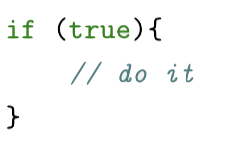
\includegraphics[scale=.6]{images/curly_braces_2.png} &  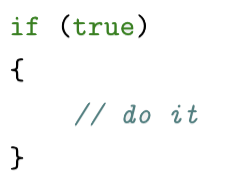
\includegraphics[scale=.6]{images/curly_braces_1.png}\\
     \tiny{Same Line} & \tiny{Own Line}\\
     \hline
 \end{tabular}
 \end{center}

And what about how to format variable names and function names:


 \begin{center}
 \begin{tabular}{| c | c | c | c | }
 \hline
    \ccb{camelCase} &  \ccb{PascalCase} & \ccb{snake\_case}  & \ccb{kebab-case}\footnote{Some languages allow the "dash" in variable names}\\
    \hline
 \end{tabular}
 \end{center}

Don't forget the mixing of rules either: "capitalize method names but not function names" and "use snake\_case for params, but not for function names", and on and on it goes. There are many many "styles" or "guides" on how to format your code. If you are interested in standardizing your programs and your own style, here is Googles \href{https://google.github.io/styleguide/cppguide.html}{style guide} for C++.

\mysubsection{Comments For Assignments}

The previous few sections are there to show you that I'm not being crazy with my expectations on comments, because there is a \textbf{whole world of crazy} when it comes to styling code. In general, my rules for comments are somewhere in between competitive programming and industry. I will give examples in the following sections, but here are my basic rules for comments: \\

\begin{enumerate}
    \item Programs get a comment block at the top ALWAYS.
    \item Functions and Classes get a comment block ALWAYS.
    \item Line up your comments!
    \item Put variable declarations on a single line and at the beginning of a code block, so you can comment each of them if needed.
    \item Place comments throughout your code giving near English explanations of your code's logic.
\end{enumerate}


\mysubsubsection{Commenting Variables}

Let's start with how I would like you to comment your variables in your code. Always place your variables at the top of the code block, on separate lines. This allows you to write a comment for each variable on its own line. Remember to line up your comments. \\
\textbf{Good}\\
\begin{minted}[]{c++}
  int num1;                 // 3 vars for users entering numbers
  int num2;
  int num3;     
  double average;           // calculated average of entered numbers
  int score1;               // score on exam 1
  int score2;               // score on exam 2
\end{minted}

\begin{minted}[]{c++}
    T **Array;          // Templated pointer to dynamic array
    int Next;           // Next available location in heap array
    int MaxSize;        // Max array size
    int HeapSize;       // Actual number of items in the array.
    bool isMax;         // true = max heap, false = min heap
\end{minted}

\textbf{Bad}\\
\begin{minted}[]{c++}
  // user  nums
  int num1, num2, num3;          
  double average;    //avg nums
  int score1,    //score exam
      score2;			    // score exam
\end{minted}

\mysubsubsection{Comment Blocks}

A comment block at the beginning of your program, a function, or a method will use the following style. VSCode has plugins to auto generate blocks for you. 

\begin{minted}[]{c++}
/**
*
* 
*
*/
\end{minted}

OR

\begin{minted}[]{c++}
/*****************************************************************************
*
* 
*
*****************************************************************************/
\end{minted}


\mysubsubsection{Program Comment Block}

The number of asterisks on the top and bottom line only matter if your writing a comment block for your program like below. The longer lines of asterisks helps create a nice visual distinction separating it from the rest of the program.\\

\textbf{Program Comment Template}\\

\begin{minted}[]{c++}
/*****************************************************************************
*                    
*  Author:           (your name)
*  Email:            (your email address)
*  Label:            (program's label from assignment list)
*  Title:            (short title from assignment, if any)
*  Course:           (course number and prefix)
*  Semester:         (semester and year)
* 
*  Description:
*        describe program here thoroughly 
* 
*  Usage:
*        how to use the program if necessary
* 
*  Files:            (list of all source files used in this program)
*****************************************************************************/
\end{minted}

\textbf{Program Comment Example}\\

\begin{minted}[]{c++}
/*****************************************************************************
*                    
*  Author:           Terry Griffin
*  Email:            terry.griffin@msutexas.edu
*  Label:            A04
*  Title:            Linked List Class
*  Course:           CMPS 3013
*  Semester:         Spring 2020
* 
*  Description:
*        This program implements a class that allows a linked list to be used just like 
*        an array. It overloads the "[]" (square brackets) to simulate accessing seperate 
*        array elements, but really it traverses the list to find the specified node using
*        an index value. It also overloads the "+" and "-" signs allowing a user to "add"
*        or "push" items onto the end of the list, as well as "pop" items off the end of our 
*        array. This class is not meant to replace the STL vector library, its simply a project
*        to introduce the beginnings of creating complex / abstract data types. 
*        
*  Usage: 
*       - $ ./main filename
*       - This will read in a file containing whatever values to be read into our list/array. 
*       
*  Files:            
*       main.cpp    : driver program 
*       list.h      : header file with list defintion
*       list.cpp    : list implementation
*****************************************************************************/
\end{minted}

\mysubsubsection{Class Comment}

\textbf{Class Comment Template}\\

\begin{minted}[]{c++}
/**
 * Class Name
 * 
 * Description:
 *      Description of your class and what it does
 * 
 * Public Methods:
 *      - A list of 
 *      - each public method
 *      - with return types
 * 
 * Private Methods:
 *      - A list of 
 *      - each private method
 *      - with return types
 * 
 * Usage: 
 * 
 *      - examples of how
 *      - to use your class 
 *      
 */
\end{minted}

\textbf{Class Comment Example}

\begin{minted}[]{c++}
/**
 * Huffman
 * 
 * Description:
 *      This class implements a compressions algorithm called Huffman Coding.
 *      Huffman coding assigns codes to characters such that the length of the 
 *      code depends on the relative frequency or weight of the corresponding 
 *      character. Huffman codes are of variable-length, and prefix-free
 * 
 * Public Methods:
 *                          Huffman()                               
 *      void                BuildFrequencyTable(string filename)
 *      string              LookupCode(char key)
 *      void                Analyze()
 *      map<char, string>   GetCodes()
 * 
 * Private Methods:
 *      void                _BuildLookupTable
 *      void                _BuildTree
 *      int                 _maxDepth
 * 
 * Usage: 
 * 
 *      Huffman H(filename):                        // Create Instance of Huffman
 *                                                  // and build freq table. 
 *      H.GetCodes();                               // get map <char,string> of codes
 * 
 *                                                  // or
 *      
 *      Huffman H;                                  // do seperately
 *      H.BuildFrequencyTable(filename);            // or use to re-build another file
 *      H.LookupCode('s')                           // get code for 's' 
 *      
 */
\end{minted}

\mysubsubsection{Function Comment}

\textbf{Function Comment Template}\\
\begin{minted}[]{c++}
    /**
     * Public/Private/Protected : function_name
     * 
     * Description:
     *      Describe the functions purpose
     * 
     * Params:
     *      - list params
     *      - one per line
     *      - with return type
     *      - and one line description
     * 
     * Returns:
     *      - what does this function return (including the type)?
     */
\end{minted}

\textbf{Function Comment Example}

\begin{minted}[]{c++}
    /**
     * Public : LoadList
     * 
     * Description:
     *      Loads an array of integers into a linked list.
     * 
     * Params:
     *      [int*]    :  array of integers
     *      [int]     :  array size
     * 
     * Returns:
     *      [type] List*   : a pointer to a linked list of integers.
     */
\end{minted}

\mysubsubsection{Code Comment Example}

\begin{itemize}
    \item Code should be commented enough to describe what is being done in general, or to clarify possibly confusing lines of code.
    \item The following is taken from a "heap" class. Knowing in general how a heap works, and by having access to the other code in the file, the comments below are enough to give the reviewer an idea of what this function is doing. 
    \item Notice that not all the comments line up, or use a single "style". I just request that your comments be consistent and neat. I chose to put some lined up to the far right, and some lined up towards the left. It's a bit of a contrived example, but I wanted to show I would accept multiple styles. 
    \item The one little pet peeve I have is that you place a space between the comment and the single line comment.
    \begin{itemize}
        \item Good: $//\;\;$This is a good comment with space after slashes.
        \item Bad: $//$This is a bad comment. No space!
    \end{itemize}
\end{itemize}

\textbf{Inline Code Comment Example}\\
\begin{minted}[]{c++}
    /**
     * public : PickChild:
     *      Return index of child to swap with or -1 to not swap.
     * 
     * Params:
     *      [int] index - index of parent element
     * 
     * Returns
     *      [int] index - index to swap with or -1 to not swap
     */
    int PickChild(int i) {
        if (RightChild(i) >= Next) {        // No right child
            if (LeftChild(i) >= Next) {     // No left child
                return -1;              
            } else {                        // There there is only a left child
                return LeftChild(i);
            }
        } else {                            // The right child exists 
            if(isMax){  
                // This is a "maxheap"
                // return child with "greater" value
                if (Array[RightChild(i)]->priority > Array[LeftChild(i)]->priority) {
                    return RightChild(i);
                } else {
                    return LeftChild(i);
                }
            }else{
                // return child with "smaller" value
                if (Array[RightChild(i)]->priority < Array[LeftChild(i)]->priority) {
                    return RightChild(i);
                } else {
                    return LeftChild(i);
                }   
            }

        }
    }
\end{minted}
